
\section{Mergeable trees} \noteauthor{Никита Елизаров}
Полное описание всех структур и доказательств можно найти в \cite{georgiadis2011data}.
\subsection{Описание структуры и чего мы хотим от этой структуры}
\begin{itemize}
    \item Храним:
    \begin{itemize}
        \item храним лес бинарных деревьев с корнем;
        \item на узлах~--- рациональные ключи;
        \item выпонено свойство кучи: $l(v)\geqslant l(p(v)).$
    \end{itemize}
    \item Поддерживаем операции:
    \begin{itemize}
        \item $parent(v)$~--- узнать, кто является предком $v$;
        \item $root(v)$~--- узнать, кто является корнем дерева, в котором находится $v$;
        \item  $nca(v, w)$~--- nearest common ancestor: если в одном дереве, то возвращает первого общего предка, если не в одном дереве, то возвращает пустое множестве;
        \item $insert(v, x)$~--- создание нового дерева с вершиной $v$ и ключом $x;$
        \item $link(v, w)$~--- подвесить $v$ к $w,$ причём $v$~--- корень какого-то дерева из леса, а у $w$ не более одного ребёнка. Также $l(v)\geqslant l(w);$
        \item $cut(v)$~--- удалить ребро между $v$ и его родителем;
       \item $delete(v)$~--- удалить $v,$ если $v$~--- лист;
       \item $merge(v, w)$~--- для начала надо сделать $link$ корней вершин, если вершины в разных деревьях. Затем мы рассматриваем два пути:
       \begin{itemize}
           \item $P$~--- путь от $v$ к корню дерева;
           \item $Q$~--- путь от $w$ к корню дерева.
       \end{itemize}
       Далее мы совмещаем эти два пути с сохранением свойства кучи. Примеры двух \textbf{merge} показаны ниже:
       \begin{center}
           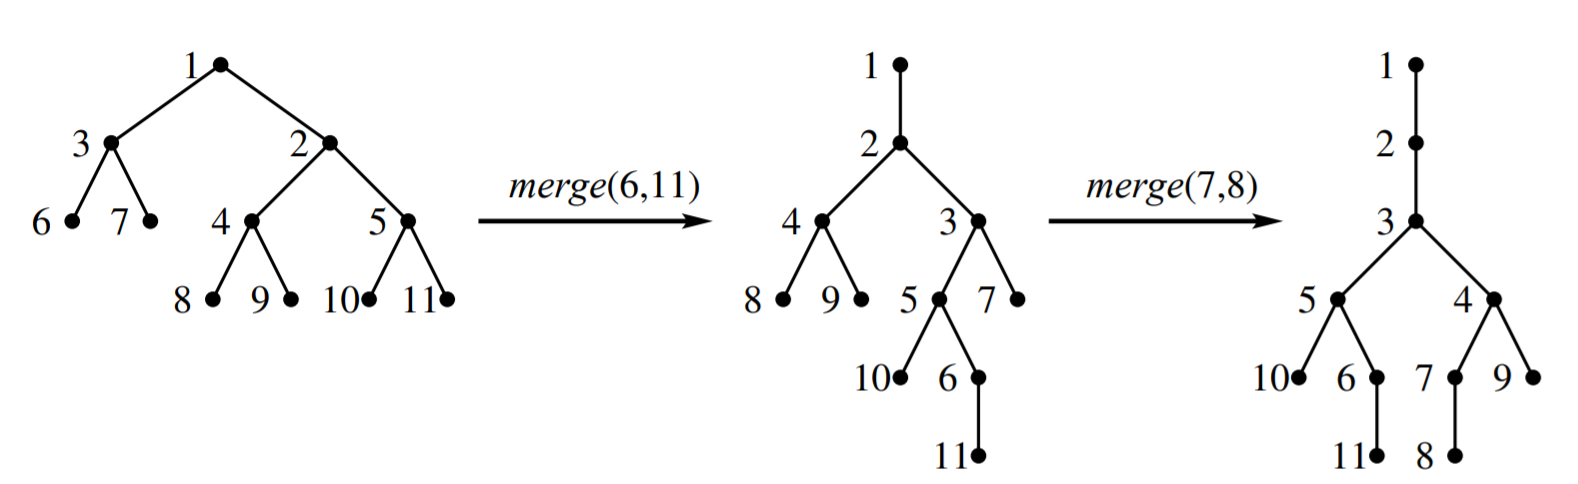
\includegraphics[scale = 0.4]{img/merge.png}
       \end{center}
    \end{itemize}
    \item Реализация.
    Реализация будет устроена так же, как и в \textbf{link-cut trees} за исключением того, что мы добавим еще одну команду \textbf{topmost}, про которую поговорим чуть позже.
    
    Заметим, что \textbf{merge} есть обобщение \textbf{link-cut}, поэтому считаем, что \textbf{link-cut} это \textbf{merge}.
    
    Введём два обозначения:
    \begin{itemize}
        \item $m$~--- количество \textbf{merge} операций к данному моменту, включая \textbf{link-cut};
        \item $n$~--- количество \textbf{insert} операций к данному моменту (начинаем с пустого дерева).
    \end{itemize}
    
    Таким образом, всё будет занимать $\mathcal{O}(n)$ памяти. 
    
    \item План.
    
    Сначала заметим, что в идеале хотим всё уметь делать за амортизированное $\mathcal{O}(\log{n}).$ Но научимся только вот так:
    \begin{itemize}
        \item если в последовательности операций над деревом есть \textbf{cut}, то умеем делать \textbf{merge} за амортизированное $\mathcal{O}(\log^2{n});$
        \item если \textbf{cut} в последовательности нет, то научимся делать за амортизированное $\mathcal{O}(\log{n});$
        \item ну а еще попутно докажем некоторые нижние оценки.
    \end{itemize}
    
\end{itemize}

\subsection{Реализация merge}
Как и оговаривалось ранее, введём операцию $\mathbf{topmost(v, w)}.$

$topmost(v,w)$~--- мы идём по пути от $v$ к $root(v),$ начиная с $v,$ и берём первую вершину $u$ такую, что $l(u) > l(w).$ Это можно сделать за $\mathcal{O}(\log{n})$ стандартным бинарным поиском.

\begin{algorithmic}[1]
    \Procedure {merge}{v, u}
        \State {u := nca(v, w)}\Comment{ищем общего предка v и w}
        \If{u = v or u = w}
            \State \Return \Comment{если общий предок совпадает с v или w, то пути уже совмещены}
        
        \Else 
            \State {x = topmost(v, u)}
            \State {y = topmost(w, u)}
            \If{x < y}
                \State {swap(x, y)}
                \State {swap(v, w)}
            \EndIf
            \If {u $\ne$ $\o$}
                \State {cut(x)}
            \EndIf
            \While {x < u}
                    \State {t := topmost(w, x)}
                    \State{link(x, parent(t))}
                    \State{cut(t)}
                    \State{y := x}
                    \State{x := t}
                    \State{swap(v, w)}
            \EndWhile
            \State {link(x, w)}
        \EndIf
    \EndProcedure
            
\end{algorithmic}
Если вершины находятся в разных деревьях, то нужно сделать еще один \textbf{link} в самом начале.

Операцию, которая находится в теле while назовём \textbf{Merge step}. Картинка к ней показана ниже:
\begin{center}
    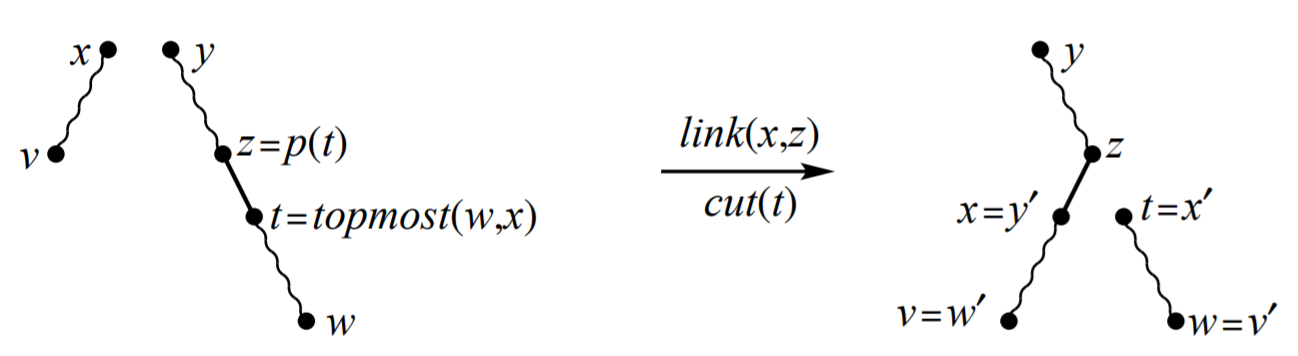
\includegraphics[scale = 0.4]{img/mergestep.png}
\end{center}

Чтобы оценить количество шагов, достаточно оценить количество изменений родителя. Поймём, что количество изменений родителя это количество merge steps плюс не более чем 2: в каждом merge step ровно одно изменение родителя, еще одно берётся в самом конце (\textbf{link(x, w)}) и еще может быть одно, если они из разных деревьев.

Теперь докажем следующую лемму.
\begin{lemma}
Количество изменений родителя это $\mathcal{O}(m\log{n}).$
\end{lemma}
\begin{proof}
Будем считать, что все наши ключи это не просто рациональные числа, а числа $\{1,\dots n\}.$ Для этого упорядочим все наши ключи в порядке возрастания и заменим каждый ключ на соответствующий номер.

$\quad$

Определим \textbf{cost} операции как количество изменений родителя. 
$$\mathbf{am.\: cost} = cost + \Delta\Phi$$
Потенциал следующий:
\begin{itemize}
    \item каждому ребру $e$ даём 1 потенциала($\Phi_e$);
    \item от каждого ребра $(parent(v), v)$ дадим $\log{(v - w)}$ родителю и $\log{(v - w)}$ ребёнку;
    \item $\Phi_v$ от вершины определяется как сумма потенциалов, которая приходит ей от рёбер (из предыдущего пункта);
    \item $\Phi = \sum\limits_{v\in V}\Phi_v + \sum\limits_{e \in E}\Phi_e.$
    
\end{itemize}
Заметим, что \textbf{cut} и \textbf{delete} уменьшают $\Phi$ хотя бы на 1 и дают не более одного изменения родителя. Значит их $\mathbf{am.\:cost} \leqslant 0.$ Остаётся только \textbf{merge}.

В начале \textbf{merge} возможен \textbf{initial link} (так как вершины могут быть в разных деревьях). Заметим, что он увеличивает потенциал не более, чем на $2\log{n} + 1:$ по логарифму в каждой вершине и 1 от ребра.

Как влияет \textbf{merge step}:
Посмотрим на родителей $t$ за два \textbf{merge step}: пусть $parent'(t)$ это родитель, который будет у $t$ на следующем \textbf{merge step} после того, который показан на картинке. Тогда:
$$t > parent'(t)\geqslant x > parent(t)$$

Первое неравенство понятно~--- это просто свойство кучи, второе чуть хитрее: новый родитель $t$ будет в ветке $y',$ то есть в ветке $x,$ но вполне может так оказаться, что это будет сам $x,$ поэтому больше либо равно. Последнее неравенство снова видно из картинки, так как $z = parent(x).$

Математической магией этих трёх неравенств получаем, что:
\begin{itemize}
    \item либо $t - parent'(t)\leqslant\frac{t - parent(t)}{2};$
    \item либо $x - parent(t)\leqslant \frac{t - parent(t)}{2}.$
\end{itemize}
В первом случае родительский потенциал $t$ уменьшается не менее чем на 1. Во втором случае детский потенциал $x$ уменьшается не менее чем на 1.

Одно из этих условий точно выполнится, а значит потенциал уменьшится хотя бы на один, таким образом (так как у нас ровно одно изменение родителя) 
$$am.\: cost(merge\:step) \leqslant 0.$$

Стоит подметить (иначе неверна строка выше), что после \textbf{initial link} все остальные изменения потенциала неположительны. Это \textbf{(!)} вроде как следует из того факта, что для $t$ его и родительский и десткий потенциал только уменьшаются (родительский - видно из неравенства, а детский, потому что на самом деле $t$ переходит в $x$, а его детский потенциал уменьшился опять же из-за этого неравенства). В итоге $t$ пробегает по всем вершинам пути (так как переходит в $x,$ а $x$ в свою очередь переходит в $y$).

Таким образом амортизационная стоимость \textbf{merge} это $\mathcal{O}(\log{n}).$ Если вспомнить, что для всех остальных операций требуется $\mathcal{O}(\log{n})$ времени, то получается, что амортизационное время работы \textbf{merge} это $\mathcal{O}(\log^2{n}).$
\end{proof}
\subsection{Merge без операций cut}
\subsubsection{Новая структура дерева}
Разбиваем деревья на сплошные пути: некоторые рёбра считаем сплошными, некоторые рёбра считаем пунктирными; компонента связности по сплошным рёбрам и есть сплошной путь.


\newdefn{
 Определим ранг вершины, как $r(v) := \bigl[\log{size(v)}\bigr],$ где $size(v)$~--- это сумма по ключам в поддереве $v,$ включая саму $v.$}

Разбивать будем следующим образом: говорим, что ребро $(v, w)$ сплошное, если $r(v) = r(w).$ \textbf{Note!} Заметим, что все таким образом определённые сплошные рёбра были бы сплошными в \textbf{link-cut} trees.

Для каждого узла будем хранить следующее:
\begin{itemize}
    \item указатель на \textbf{parent(x)};
    \item указатель на \textbf{solid child(x)} (то есть указатель на ребёнка, соединённого сплошным ребром, если такой есть);
    \item указатель на \textbf{head(x)}~--- отдельная вершина, в которой хранится указатель начало сплошного пути, в котором вершина находится;
    \item \textbf{dashed size(x)} $:= 1 + \sum\limits_{u \text{~--- пунктирный ребёнок}}size(u)$
\end{itemize}
Такая структура двухсвязного списка позволяет ускорить операции вставки и удаления.

Также, для каждого сплошного пути мы будем хранить следующее:
\begin{itemize}
    \item \textbf{head(x)}~--- отдельная вершина, в которой хранится указатель на \textbf{top} пути, а также размер \textbf{top} и ранг всего пути;
    \item поисковая структура~--- пока структура, которая будет уметь выполнять три функции:
    \begin{itemize}
        \item удалять узлы в начале пути за $\mathcal{O}(1)$;
        \item добавлять одиночные узлы перед заданным за $\mathcal{O}(1)$;
        \item делать \textbf{topnode(x, s)}~--- наименьший узел на сплошном пути, содержащим $s,$ ключ которого больше чем $x.$
    \end{itemize}
    \item более того, каждый \textbf{head} хранит указатель на поисковую структуру соответствующуего сплошного пути.
\end{itemize}

Тот факт, что мы храним только размер top пути, позволяет нам пересчитывать все остальные размеры, пользуясь формулой:
$$size(x) = size(p(x)) - d(p(x)).$$


\subsubsection{Стэк $S_v$}
Теперь root(v) возвращает стек начал сплошных путей, которые находятся на пути $[v, root(v)].$
Эти стеки полезны в нахождении \textbf{nca(v, w)}.  Для начала, найдём два стека для $v, w$ соответственно (обозначим их за $S_v$ и за $S_w$). А далее:

\begin{algorithmic}[1]
\Procedure{nca}{v, w}
    \If{$top(S_w)\ne top(S_v)$}
        \State\Return {0}
    \Else
        \While{$top(S_v) = top(S_w)$}
            \State {$pop(S_v$)}
            \State {$pop(S_w)$}
        \EndWhile
        \If{$S_v = S_w = \varnothing$}
            \State\Return{min\{$v, w$\}}
        \EndIf
        \If {$S_v = \varnothing$ and $S_w\ne\varnothing$}
            \State\Return {min\{$v, p(top(S_w))$\}}
        \EndIf
        \If {$S_v \ne \varnothing$ and $S_w = \varnothing$}
            \State\Return {min\{$w, p(top(S_v))$\}}
        \EndIf
        \If {$S_v \ne \varnothing$ and $S_w\ne\varnothing$}
            \State\Return {min\{$p(top(S_v)), p(top(S_w))$\}}
        \EndIf
    \EndIf
\EndProcedure
\end{algorithmic}
Так как рангов всего не более $\log{n},$ то видно, что \textbf{nca} работает за $\mathcal{O}(\log{n}).$

$\quad$

\subsubsection{Link}
Теперь поговорим про \textbf{link(v, w)}. Проделывать мы будем его в несколько этапов:
\begin{itemize}
    \item добавляем ребро $(v, w),$ сначала как пунктирное;
    \item ищем множество узлов, где ранг меняется. Обозначим его за $Q.$ Утверждается, что $Q$ представляет собой объединение начал сплошных путей. Поэтому искать мы $Q$ будем поднимаясь в \textbf{head} пути и спускась, пока ранг отличается от старого.
    \item все сплошные выходящие рёбра из вершин из $Q$ заменить на пунктирные, пересчитать ранг;
    \item меняем обратно те пунктирные, которые должны быть сплошными; (Здесь возникает проблема, так как нам надо следить за добавлением вершин в поисковую структуру пути)
\end{itemize}
\begin{lemma}
Суммарное время на все операции \textbf{link} это $\mathcal{O}(m\log{n}).$
\end{lemma}
\begin{proof}
Можем оценить время работы как константа умножить на количество вставок в $Q$ или в $S_w.$ Заметим, что если мы вставляем вершину в $Q,$ то в итоге вставляем и в $S_w$ (когда мы меняем сплошные рёбра на пунктирные; здесь мы можем считать, что мы просто добавляем их в $S_w$). 

Также в самом начале мы вызывали \textbf{root(w)} и поэтому мы добыли $S_w$ размера $\mathcal{O}(\log{n}).$ Заметим, что при добавлении вершины в $S_w$ её ранг увелиличился. Так как ранг для каждой вершины увеличился не более чем на $\mathcal{O}(\log{n})$ раз и $m > n,$ то общее время работы не более $\mathcal{O}(m\cdot\log{n}).$ \textbf{Важно!} Так как у нас нет cut, то ранги только растут.
\end{proof}
\subsubsection{Merge}
\begin{itemize}
    \item сначала мы снова заботимся о том, чтобы обе вершины оказались в одном дереве, делая \textbf{link};
    \item в остальном делаем merge также как и в прошлой подсекции (что мы делаем с обновлением структур поймём позже)
    \begin{center}
        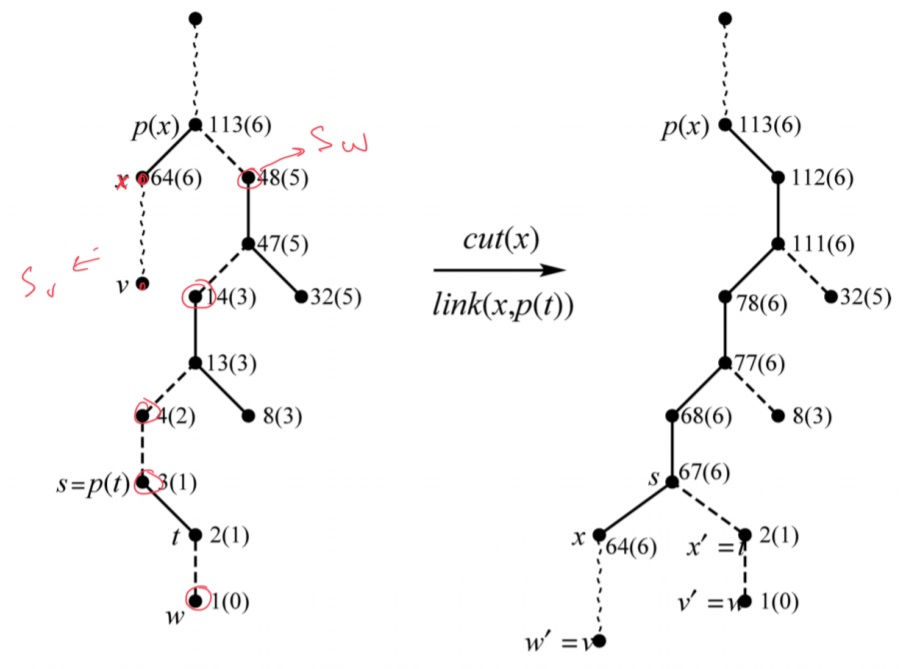
\includegraphics[scale = 0.6]{img/new_merge.jpg}
    \end{center}
    \item \textbf{(?)} утверждается, что понимать, куда именно вставлять вершины мы будем уметь, используя структуру на путях (которую мы еще не ввели) и \textbf{topnode}.
    
\end{itemize}
\begin{lemma}
Не считая вызовов \textbf{topnode}, затраченное время на все \textbf{merge} не превосходит $\mathcal{O}(m\cdot\log{n}).$
\end{lemma}
\begin{proof}
Во время одного merge мы возможно соединяем два дерева с помощью \textbf{link}. Это мы делаем за амортизированный $\mathcal{O}(\log{n}).$ 

Из первой подсекции мы знаем, что количество \textbf{merge steps} это $\mathcal{O}(m\cdot\log{n}.)$ Во время \textbf{merge step} мы достаем из $S_v$ и $S_w$ и добавляем в $Q.$ Как и в прошлой лемме, в начале мы добавили в $S_v$ и $S_w$ по $\mathcal{O}(\log{n})$ вершин, а последующие добавления снова лишь увеличивают ранг, а так как у каждой вершины не более $\mathcal{O}(\log{n})$ увелечений ранга, то мы снова получаем $\mathcal{O}(m\cdot\log{n}).$ \textbf{Важно!} Так как у нас нет \textbf{cut}, то ранги только растут.

\end{proof}
\subsubsection{Поисковая структура на путях}
Также как и в \textbf{link-cut trees} мы будем представлять сплошной путь в виде \textbf{splay-дерева}.

Будем доказывать, что в \textbf{splay-дереве topnode} запрос можно сделать за $\mathcal{O}$(\textbf{parent change}), где \textbf{parent change} следует за запросом \textbf{topnode}.

\newdefn{Finger~--- узел, посещённый в splay-дереве последний раз.}

Результат без доказательства: \textbf{am. cost} (операций со \textbf{splay-деревом}) это $\mathcal{O}(\log{d + 1}),$ где $d = |f' - f|$ \textbf{(?)} Здесь, $f'$ и $f$~--- новый и старый \textbf{finger} соответственно.
\newdefn{$\log{d + 1}$~--- время Коула для данной операции.}
\begin{lemma}
Добавление посещения узла между операциями не уменьшает время Коула.
\end{lemma}
\begin{proof}
Самостоятельно (утверждается, что несложно).
\end{proof}

Предпологается, что можно доказать, что \textbf{topnode} работает за $\mathcal{O}$(\textbf{parent change}) без модификаций, но это открытый вопрос, поэтому мы модифицируем: когда хотим что-то добавить в сплошные пути во время работы \textbf{merge}, мы добавляем не сразу а при случае (позволяется иметь узы в сплошном пути не в \textbf{splay-дереве}).

Тогда реализация \textbf{topnode(x,e)} выглядит следующим образом: мы делаем бинарный поиск $e$ в \textbf{splay-дереве}. Тогда ответом будет являться:
\begin{itemize}
    \item либо последний посещённый узел в бинарном поиске;
    \item либо сплошной ребёнок последнего посещённого узла;
    \item либо вершина, которая находится не в дереве.
\end{itemize}
Если это либо первая, либо вторая ситуация, то \textbf{(?)} всё хорошо, мы нашли и делаем \textbf{splay}. Если же это третья ситуация, то мы остановились в самой правой нижней вершине, обозначим её за $y$, делаем \textbf{splay(y)}, а далее просто идём по указателям по вершинам и последовательно находим \textbf{topnode}. Пока мы идём до нашего результата и находим что-то новое~---добавляем это в \textbf{splay-дерево}.

$\quad$

Далее будет описана идея доказательства, что \textbf{topnode} работает за $\mathcal{O}$(\textbf{parent change}) (автор конспекта не очень понял на момент написания, для полного понимания нужно прочитать почти всю статью):

На \textbf{topnode} требуется $\mathcal{O}(1)$ + количество операций со \textbf{splay-деревом} (ну и время на эти операции).

Определим потенциал и \textbf{am. cost}:

Пусть $d_f$~--- количество предков $f$ на сплошном пути. Тогда потенциал дерева $\Phi_T = \log{d_f},$ где $f$~--- это \textbf{finger} дерева. Потенциал всей системы это $\sum\limits_{T\in M}\Phi_T.$

\textbf{am.cost} операций со \textbf{splay-деревом} = время Коула + увеличение потенциала. 

Также перед любым \textbf{merge} мы "просто потрогаем \textbf{top} пути." \textbf{Важное замечание.} Если мы хотим что-то делать с \textbf{top} пути, то это будет за $\mathcal{O}(1),$ так как время Коула уравновешивается изменением потенциала. Если мы хотим что-то делать на расстоянии $\mathcal{O}(1)$ от предыдущего узла, то тоже делается за $\mathcal{O}(1).$ Из чего следует, что \textbf{delete} и \textbf{insert} из \textbf{top}, в \textbf{top}, либо рядом с предыдущим \textbf{finger} тоже делается за $\mathcal{O}(1).$

Из всего этого мы можем заключить, что суммарная стоимость на \textbf{merge} $\mathcal{O}(m\cdot \log{n})$ за исключением \textbf{access}.

\textbf{Access}: разбор случаев, но в каждом случае \textbf{am.cost} $\leqslant 2\cdot \mathbf{cost(query)} + \mathcal{O}(1),$ где \textbf{cost(query})~--- изменение родителей.

